\documentclass[12pt]{article}
\usepackage{amsmath, amssymb, graphicx, setspace, color, physics, nicefrac, float}
\usepackage[utf8]{inputenc}
\usepackage[numbers]{natbib}
\usepackage[colorlinks, citecolor = blue, urlcolor = blue]{hyperref}
\usepackage[makeroom]{cancel}
\setlength\parindent{0pt}

\newcommand{\answer}[1]{\underline{\underline{#1}}}
\renewcommand{\d}[1]{\ensuremath{\operatorname{d}\!{#1}}}
\newcommand{\R}{\mathbb{R}}
\newcommand{\C}{\mathbb{C}}
\newcommand{\Z}{\mathbb{Z}}
\newcommand{\Q}{\mathbb{Q}}
\newcommand{\tenmix}[3]{{#1}^{#2}_{#3}}
\newcommand{\vectorproj}[2][]{\textit{proj}_{\vect{#1}}\vect{#2}}


\title{INF-1400 Assignment 1 \\ Report} 
\author{Lasse Treten}

\begin{document}
\maketitle
\clearpage
    \section{Introduction}
        In this assignment I have implemented a version of the classic arcade game, Breakout \citep{breakout}. The game was originally developed by Atari inc, and released May 13, 1976.
        
    \section{Background}
        This project were implemented using python 3.8.1 \cite{pythonversion} with an extensive use of the pygame library \cite{pygame}.\\
        All graphical content were downloaded from OpenGameArt.org \cite{opengameart, breakout_graphics,  lava_graphics}, which is a media repository intended for free and open source game projects. 

    \section{Design}
        Almost all of the content that appears on screen are build around pygame's Sprite class \cite{Sprite}. This class provides a comprehensible interface, which makes it effortless to draw objects, updating positions, and creating hit boxes. \\
        I have chosen to create a subclass called ``SpriteMe'', which takes in a pygame.Surface, creates a hit box around it, and returning it as a sprite. From this class there are tree derived sub classes, see figure \ref{UML}.
    
        \begin{figure}[H]
            \centering
            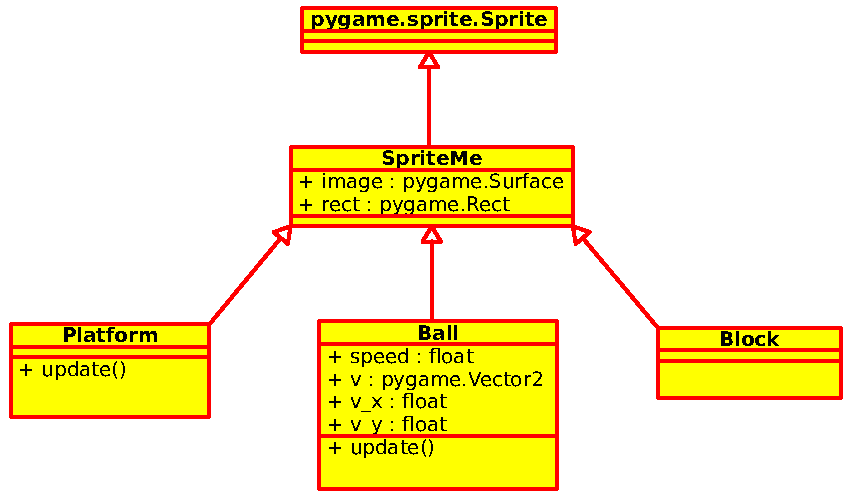
\includegraphics[scale = 0.8]{uml.eps}
            \caption{UML}
            \label{UML}
        \end{figure}
    
    \section{Implementation}
        The Project is seperated into two different files, breakout and spriteloader. 
        Classes, methods and functions are documented through doc-strings. Some more thorough than other. \\
        The two classes "SpriteMe" and "SpriteSheet" are defined in the spriteloader file. The latter handles so called spritesheets, which is a single image file containing multiple figures. It has a method called get\_sprite, which picks out a figure from the sheet and loads it as a pygame.Surface. This organizes graphics in a neat way, saving space.\\
        
        
        The Ball, Platform and Block classes are defined in the breakout file, along with a couple of functions that places and organize instances. It is also here the game loop is implemented. 
        
        
            \subsection{Collision handling}
                A crucial part of game development is to handle interactions between object appearing on the screen. In our game we have two key interactions, the ball hitting the blocks, and the ball hitting the platform. In both cases the ball needs to change it's motion. \\ 
                When the ball collides with one or more of the blocks, the vertical component of the velocity, ball.v\_y is reflected. \\
                The interaction between the ball and the platform is a little more subtle. We want the motion of the ball to depend on were it hits the platform. In particular, if the ball hits on the left side of the platform the new motion will be to the left, and if it hits at the center the motion will be vertical. How much the direction will change is dependent on how far toward either of the edges the collision appears. I have come up with the following model. \\[2mm]
                Let $ v $ be the unit normal vector for the balls' velocity after a collision with the platform is detected. $ v $ is defined by
                \begin{align}
                    & v(d) = \left( \cos \left(\frac{\left(m - \alpha d \right)\pi}{2m} \right),  \sin \left(\frac{\left(m - \alpha d \right)\pi}{2m} \right)\right) 
                \end{align}
               $ d $ is the horizontal difference for the balls' center and the platforms' center.\\
               $ m $ is the maximal difference possible, in other words, $ d \in [-m, m] $. \\
               $ \alpha \in [0, 1] $ is a parameter which determines how drastic the change in motion shall be. For $ \alpha = 0 $ the ball will bounce vertical upwards, no matter were on the platform it hits. For $ \alpha = 1 $ the ball will travel horizontal if it hits at the edges.
               Positive vertical motion is defined upwards. \\
               The detection of sprites colliding is done through the sprite.spritecollide method, see  \cite{Sprite} for documentation. This method makes use of the rect attribute inherited from SpriteMe. 
               
        \section{Evaluation} 
            The game fulfills the requirements in the assignment. That said, there are room for improvements. 
            
        \section{Discussion}
            Even dough the game has all the key ingredients, there are a lot more features that could have been added. For instance, a score board and different levels.\\
            
            The collision detection relies solely on the spritecollide method, which again is based on the rect.colide method. This solution works fine for objects that are shaped like a rectangle, like the platform and the blocks. The ball on the other hand, should properly had a circular hit box, though in this game such precision is not crucial. \\
            Also one could have implemented a more sophisticated motion after the ball have collided with the blocks. Here there are different options that could have added more dept into the game. 
                
        \section{Conclusion}
            This project got to demonstrate many key aspects of object oriented programming, such as inheritage and choice of design (API). It also were a fine introduction to basic game development and the pygame library. 


\bibliographystyle{plainnat}
\bibliography{assignment1_INF-1400}
\end{document} 
